\section{Resumen}

	\hspace{1cm}Es interesante plantearse cu\'ando se requiere la utilizaci\'on de m\'etodos num\'ericos para la resolución de problemas, en este caso ecuaciones diferenciales ordinarias (en el tratado del presente trabajo). No sólo se las utiliza cuando las soluciones analíticas no pueden ser expresadas por las clásicas funciones fundamentales; sino que a su vez se tiene como ejemplo el paper del que se tomaron las EDOs que se estudian en este trabajo práctico, en donde se expone otra razón para la utilización de análisis numérico: a boca del propio autor, comenta que en el estado estacionario la solución analítica para encontrar la raíz consiste en más de 200 términos con los que realizar álgebra, haciéndolo engorroso en la práctica. Además pueden generar errores numéricos ligados a las operaciones algebraicas en representación de tipo float. Por ende, en este caso, se optó por encontrar las raíces de forma numérica, conociendo previamente que el sistema tiene un único punto fijo en la región local del espacio parametrizado explorado (Model Analysis and Simulation Results en el paper).

\hspace{1cm}Tras reconocer que Heun está contenido en el segundo orden de Runge-Kutta, resulta entonces como pregunta natural cuestionarse cuándo es conveniente parar de escalonar en el orden, es decir, cuándo la eficiencia empieza a bajar de manera mucho más marcada en contraposición a la precisión lograda. La respuesta en realidad depende de la naturaleza del problema. Pero como regla general (obviamente existen excepciones), es conveniente usar un orden mayor cuando se está muy limitado a errores de redondeo, porque mayor orden requiere menos pasos. Es decir, menos evaluaciones de funciones, cuentas, y demás). En este trabajo se usó Heun por consigna.

\hspace{1cm}Se comenta brevemente la manera de aproximar de Heun, que se ve reflejada los códigos m\'as adelante. La misma es un modelo superador de Euler, de mayor precisión. Euler lo que hace es tomar la línea tangente a la función al principio del intervalo asumiendo que el paso es suficientemente chico como para aproximar a la tangente. Sin embargo, aún cuando el paso sea verdaderamente muy chico, el error se va acumulando en muchos casos considerablemente. Heun considera las líneas tangentes a la curva solución en ambos puntos que limitan el intervalo, uno que subestima y otro que sobreestima la coordenada vertical ideal, y sobre ellos realiza una ponderación equitativa. En el propio método se nota que la piedra fundacional del algoritmo está emprendida por Euler como pionero.

\hspace{1cm}Bas\'andonos en el desarrollo num\'erico del art\'iculo de \textit{Lemaire et al. [1]: "Modeling the interactions between osteoblast and osteoclast activities in bone remodeling" }, en este trabajo se resuelven las siguientes ecuaciones diferenciales ordinarias implementando el m\'etodo de Heun.
$$ \frac{dR}{dt} = D_R . \pi_C - \frac{D_B}{\pi_C} . R + I_R$$
$$ \frac{dB}{dt} = \frac{D_B}{\pi_C} . R - k_B . B + I_B$$
$$ \frac{dC}{dt} = D_C . \pi_L - D_A . \pi_C . C + I_C$$

\hspace{1cm}Las constantes de estas ecuaciones se encuentran especificadas en el Paper mencionado. A partir de estas tres ecuaciones diferenciales ordinarias, se graficaron nueve figuras 	que cumplen con los par\'ametros especificados en el enunciado de la consigna del presente trabajo pr\'actico.


\section{Implementaci\'on}

\hspace{1cm}Sobre cuestiones ligadas a la implementación: se usó un método iterativo para encontrar el máximo error absoluto admisible. El mismo no es de los más eficientes que se pudieron haber implementado ya que, por ejemplo, podría haberse aumentado el orden de eficiencia realizando una búsqueda binaria para localizar un intervalo chico. Sin embargo, no se lo consider\'o algo que amerite demasiado trabajo de optimización, porque no logra una mejora sustancial y de esta forma el código resulta más legible, por lo que se eligió este último criterio. A continuaci\'on se presentan los c\'odigos implementados para obtener los gr\'aficos que se encuentran m\'as abajo.

\begin{lstlisting}[language=Matlab, caption=heun.m]
function [x t]=heun(f,x0,t0,tf,n,par)
    h=(tf-t0)/n;
    t=linspace(t0,tf,n);
    x(1,:)=x0;
    for i=1:n-1
        k1(i,:)=f(t(i),x(i,:), par);
        k2(i,:)=f(t(i)+h,x(i,:)+k1(i,:), par);
        x(i+1,:)=x(i,:)+(h/2)*(k1(i,:)+k2(i,:));
    end
\end{lstlisting}

\begin{lstlisting}[language=Matlab, caption=miode.m]
function [x t]=miode(f,x0,t0,tf,dtmax,tol,par)
  n = ceil((tf-t0)/dtmax);
  err = 1;
  
  while (err > tol)
    [x1 t1] = heun(f,x0,t0,tf,n,par); 
    [x2 t2] = heun(f,x0,t0,tf,n*2, par);
    err = max(abs(x1(tf)-x2(tf)));
    n = n + 1;
  end
  
  [x t] = heun(f,x0,t0,tf,n-1,par); 
\end{lstlisting}

\begin{lstlisting}[language=Matlab, caption=ejemplo.m]
f=@(t,y,p) 2*t;

[x t] = miode(f, 1, -2, 2, 1, 10^-1,'a');

plot(t,x)
\end{lstlisting}

\begin{lstlisting}[language=Matlab, caption=edos.m]
clear all;
clc;

I_R=@(t,p) strcmp(p,'a3')*(0.0001).*(20<=t && t<=80)+strcmp(p,'b3')*(-0.00012).*(20<=t && t<=80);

I_B=@(t,p) strcmp(p,'a1')*(0.0001).*(20<=t && t<=80)+strcmp(p,'b1')*(-8.3*10^-5).*(20<=t && t<=80);

I_C=@(t,p) strcmp(p,'a2')*(0.0001).*(20<=t && t<=80)+strcmp(p,'b2')*(-0.00029).*(20<=t && t <= 80);

I_P=@(t,p) strcmp(p,'c1')*(1000).*(20<=t && t<=80);

I_0=@(t,p) strcmp(p,'c2')*(2.5*10^5).*(20<=t && t<= 80);

I_L=@(t,p) strcmp(p,'c3')*(10^4).*(t>=20);

% constantes
k1 = 10^(-2);
k2 = 10;
f0 = 0.05;
d_B = 0.7;
Cs = 5*10^(-3); 
k3 = 5.8 * 10^(-4);
k4 = 1.7 * 10^(-2);
k0 = 0.35;
K = 10;
klp = 3*10^6;
kop = 2*10^5;
r_L = 10^3;
k_P = 86;
S_P = 250;
k6 = 3;
k5 = 0.02;

P0 = S_P / k_P;
Ps = k6 / k5;

D_R = 7*10^(-4);
D_B = f0 * d_B; 
k_B = 0.189;
D_C = 2.1*10^(-3);
D_A = 0.7;
R = 0.0007734;
B = 0.0007282;
C = 0.0009127;

pi_C = @(t,y,p) (y(3) + f0 * Cs)/(y(3) + Cs);
P_ = @(t,p) I_P(t,p) / k_P;
pi_p = @(t,p) (P_(t,p) + P0)/(P_(t,p) + Ps);
pi_L = @(t,y,p) (k3/k4)*((klp * pi_p(t,p) * y(2))/(1 + (k3*K/k4) + (k1/(k2*k0))*(((kop/pi_p(t,p))*y(1)) + I_0(t,p) ))) * (1 + (I_L(t,p)/r_L));


f=@(t,y,p)[
    D_R*pi_C(t,y,p)-(D_B/pi_C(t,y,p))*y(1)+I_R(t,p),D_B/pi_C(t,y,p)*y(1)-k_B*y(2)+I_B(t,p),D_C*pi_L(t,y,p)-D_A*pi_C(t,y,p)*y(3)+I_C(t,p)
   ];


[x t] = miode(f, [R B C], 0, 140, 1, 10^-6,'a1');
plot(t, x)
[x t] = miode(f, [R B C], 0, 140, 1, 10^-6,'a2');
plot(t,x)
[x t] = miode(f, [R B C], 0, 140, 1, 10^-6,'a3');
plot(t,x)
[x t] = miode(f, [R B C], 0, 140, 1, 10^-6,'b1');
plot(t,x)
[x t] = miode(f, [R B C], 0, 140, 1, 10^-6,'b2');
plot(t,x)
[x t] = miode(f, [R B C], 0, 140, 1, 10^-6,'b3');
plot(t,x)
[x t] = miode(f, [R B C], 0, 140, 1, 10^-6,'c1');
plot(t,x)
[x t] = miode(f, [R B C], 0, 140, 1, 10^-6,'c2');
plot(t,x)
[x t] = miode(f, [R B C], 0, 140, 1, 10^-6,'c3');
plot(t,x)

\end{lstlisting}

\section{Resultados}

\hspace{1cm}Aqu\'i se pueden observar gr\'aficamente las soluciones de las EDOs, como se mencion\'o previamente. Sus nombres $a1, a2, a3, b1, b2, b3, c1, c2 y c3$ son consistentes con las indicaciones de los par\'ametros presentes en la consigna del trabajo pr\'actico.
\begin{figure}[h!]
\centering
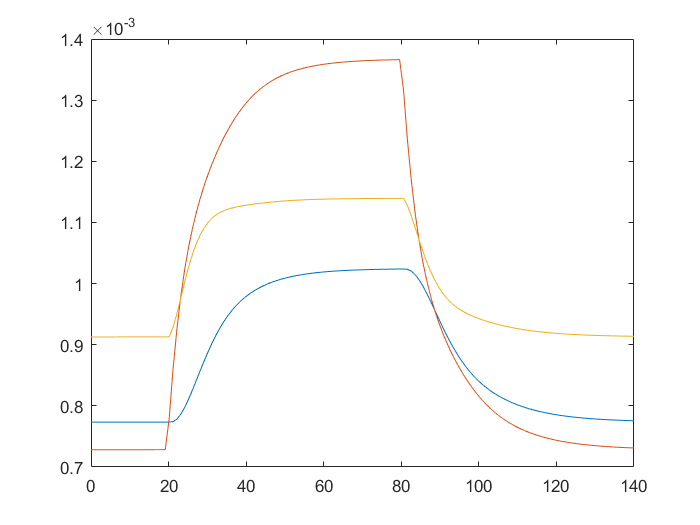
\includegraphics[scale=0.3]{../a1.png}\hspace{0.01cm}
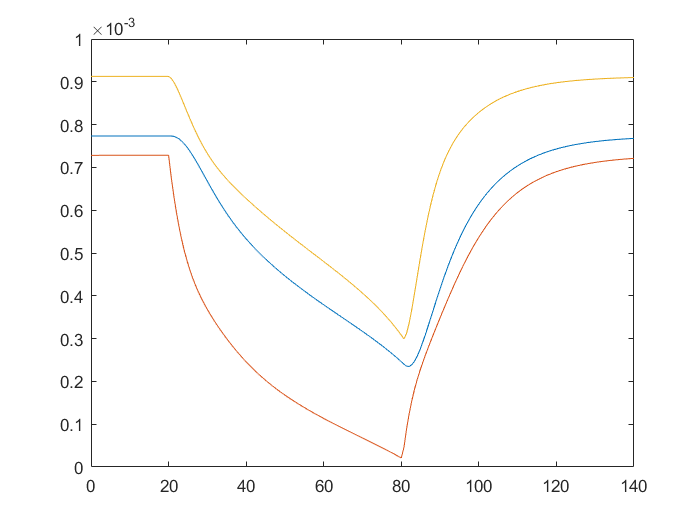
\includegraphics[scale=0.3]{../b1.png}\hspace{0.01cm}
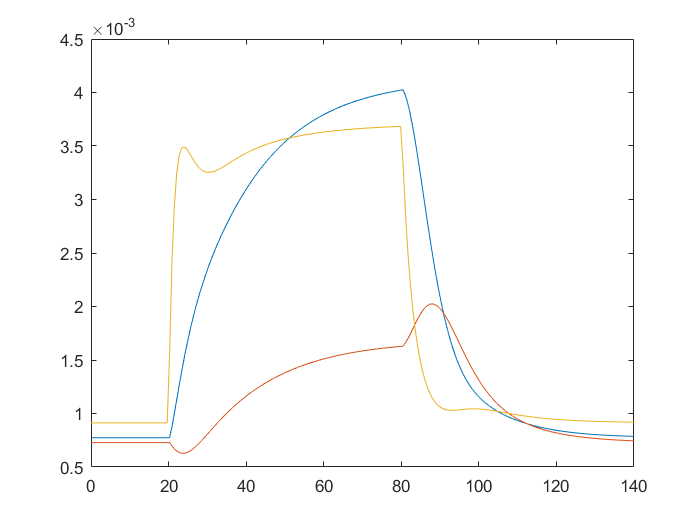
\includegraphics[scale=0.3]{../c1.png}\\
\caption{Figuras $a1, b1 y c1$ respectivamente.}
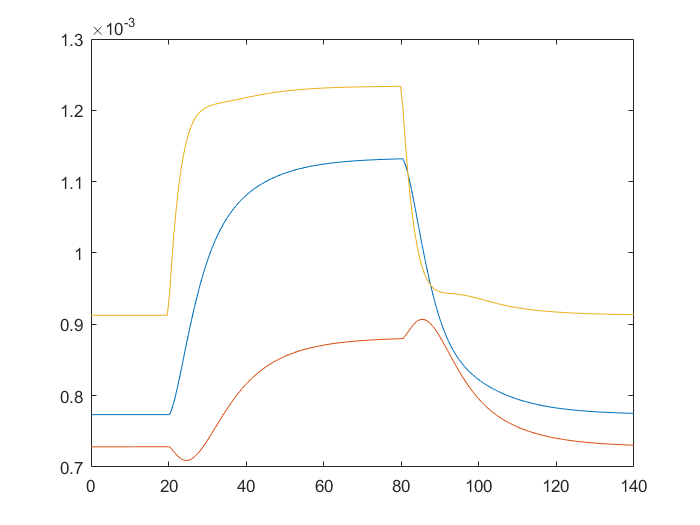
\includegraphics[scale=0.3]{../a2.png}\hspace{0.01cm}
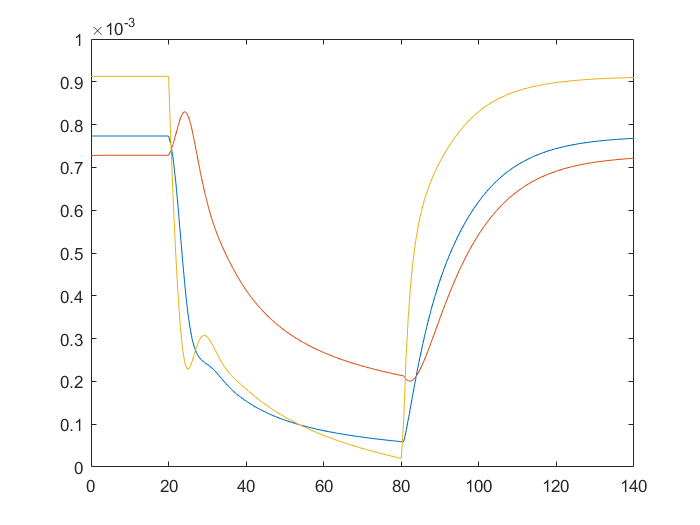
\includegraphics[scale=0.3]{../b2.png}\hspace{0.01cm}
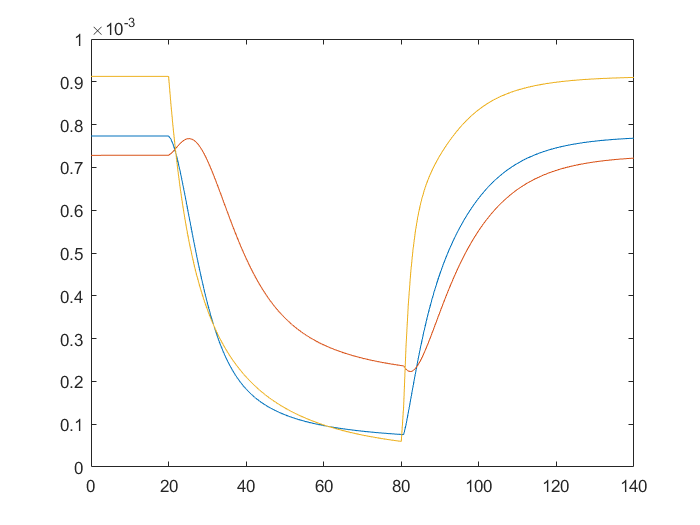
\includegraphics[scale=0.3]{../c2.png}\\
\caption{Figuras $a2, b2 y c2$ respectivamente.}
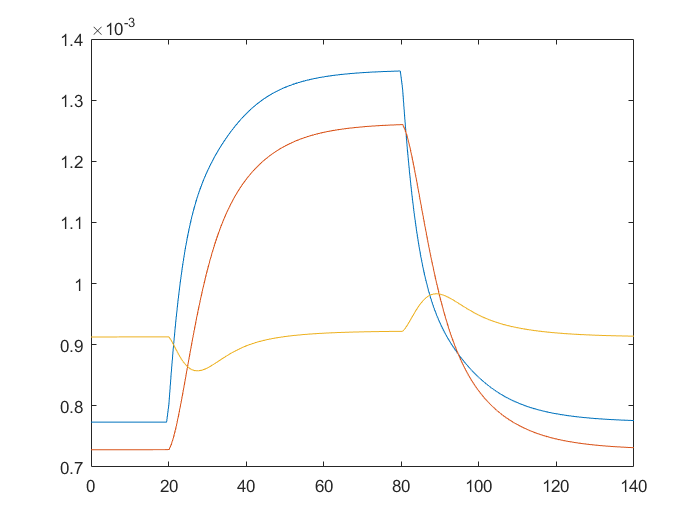
\includegraphics[scale=0.3]{../a3.png}\hspace{0.01cm}
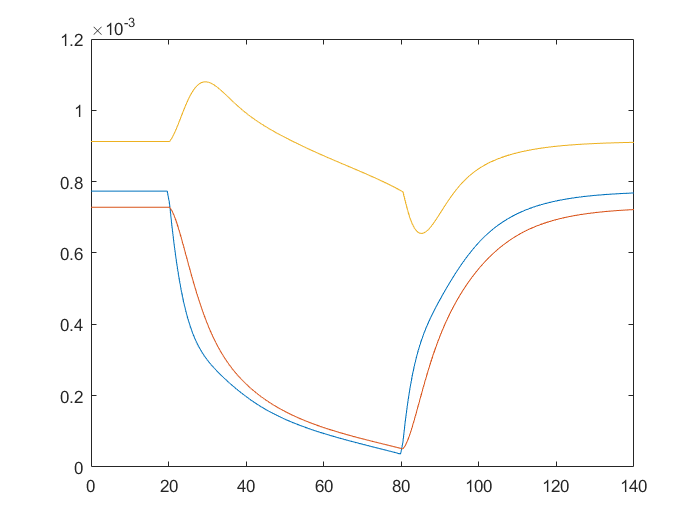
\includegraphics[scale=0.3]{../b3.png}\hspace{0.01cm}
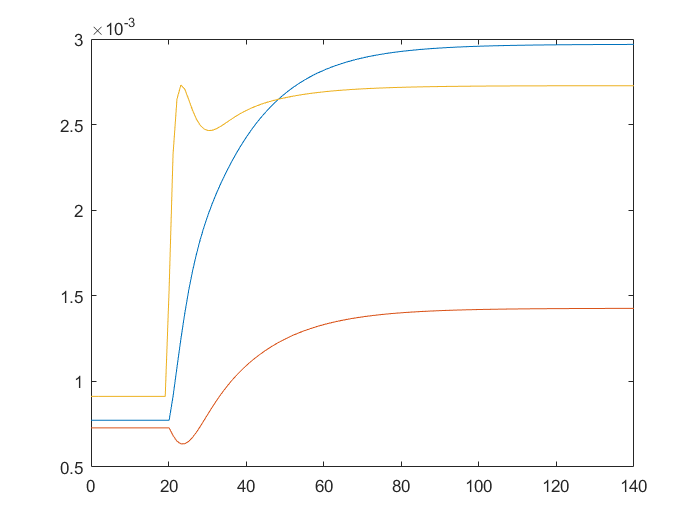
\includegraphics[scale=0.3]{../c3.png}
\caption{Figuras $a3, b3 y c3$ respectivamente.}
\caption{Resultados de las EDOs.}
\label{circnpnmaxout}
\end{figure}

Se puede observar que los gr\'aficos se ven como los del Paper mencionado.


